\documentclass[10,a4paperpaper,]{article}

  \title{Reporte de encuestas electorales}
  \author{Gerencia del Poder}
  \date{\today}
  


\newcommand{\logo}{logo.png}
\newcommand{\cover}{cover.png}
\newcommand{\morena}{751438}
\newcommand{\amarillom}{ba9f19}
\usepackage{booktabs}
\usepackage{longtable}
\usepackage{array}
\usepackage{multirow}
\usepackage{wrapfig}
\usepackage{float}
\usepackage{colortbl}
\usepackage{pdflscape}
\usepackage{tabu}
\usepackage{threeparttable}
\usepackage{threeparttablex}
\usepackage[normalem]{ulem}
\usepackage{makecell}
\usepackage{xcolor}

% Author: Karol KozioL and Jaziel Flores
% License: GPL-3
% Modified by: Sarah Wagner

% % % packages -----------------------------------------------------------------------------------
\usepackage{amsmath}
\usepackage{array}
\usepackage{booktabs}
\usepackage{calc}
\usepackage{eso-pic}
\usepackage{fancyhdr}
\usepackage{fontspec}
\usepackage[left = 2.5cm, right = 2.5cm, top = 1.2cm, bottom = 1.2cm, includeheadfoot]{geometry}
\usepackage{graphicx}
\usepackage[utf8]{inputenc}
\usepackage{lastpage}
\usepackage{multirow}
\usepackage{tabularx} 
\usepackage{tikz}
\usepackage{titlesec}
\usepackage{xcolor, colortbl}

% % % settings -----------------------------------------------------------------------------------

% % custom colors
\definecolor{iblue}{HTML}{\iblue}
\definecolor{igray}{HTML}{\igray}

\definecolor{morena}{HTML}{751438}
\definecolor{amarillom}{HTML}{ba9f19}

% definition of pagename
\newcommand\pagename{Page}

% % fonts 
\defaultfontfeatures{Mapping = tex-text}
\setmainfont[BoldFont = Poppins-Bold.ttf, ItalicFont = Poppins-Italic.ttf, BoldItalicFont = Poppins-BoldItalic.ttf]{Poppins-Regular.ttf}
  \newfontfamily\headingfont[ItalicFont = Poppins-BlackItalic.ttf]{Poppins-Black.ttf}


% % sections
\titleformat{\section}{\color{iblue}\headingfont\Large\bfseries}{\thesection}{1em}{}[\titlerule]
\titleformat{\subsection}{\color{iblue}\headingfont\large\bfseries}{\thesubsection}{1em}{}
\titleformat{\subsubsection}{\color{iblue}\headingfont\bfseries}{\thesubsubsection}{1em}{}

% % misc
\setlength{\parindent}{0em} 
\linespread{1}
\raggedright
\newcolumntype{C}{>{\centering\arraybackslash}X}


% % % custom titlepage ----------------------------------------------------------------------------
\newcommand\BackgroundPic{%
	\put(0,0){%
		\parbox[b][\paperheight]{\paperwidth}{%
			\vfill
			\centering
			
\includegraphics[width=\paperwidth,height=\paperheight]{\cover}%
			\vfill
}}}

\makeatletter

% pagestyle titlepage
\fancypagestyle{customtitle}{
	\lhead{}
	\chead{}
	\rhead{}
	\makeatother
	\lfoot{}
	\cfoot{}
	\rfoot{
\includegraphics[width=4cm,height=1.2cm]{\logo}}
}


% titlepage
\renewcommand{\maketitle}{
	\thispagestyle{customtitle}
	\AddToShipoutPicture*{\BackgroundPic}
	\ClearShipoutPicture
	
	\phantom{a}\hfill
	\vspace{14cm}
	
	\begin{tabular}[l]{@{}p{\textwidth}@{}}
		\color{morena}\headingfont\LARGE\@title\\[1em]
		\color{morena}\headingfont\large\@author\\[1em]
		\color{morena}\headingfont\small\@date\\[1em]
	\end{tabular}
	
	
	
	\clearpage
}
\makeatother

% % % header and footer ---------------------------------------------------------------------------
\pagestyle{fancy}
\lhead{}
\chead{}
\rhead{ 
\includegraphics[width=4cm,height=1.2cm]{\logo}}
\makeatother
\newlength{\myheight}
\lfoot{}
\cfoot{}
\rfoot{\pagename~\thepage \hspace{1pt} / \pageref{LastPage}}
\renewcommand\headrulewidth{0pt}
\renewcommand\footrulewidth{0pt}




\begin{document}


\renewcommand{\contentsname}{Gerencia del Poder}

\renewcommand{\pagename}{Página}


\maketitle
\tableofcontents
\addcontentsline{toc}{section}{Contenido}
\clearpage

\section*{Reporte de Cuestionarios}

\begin{center}
  \begin{tabular}{ c  c }
    \begin{mybox}[colback=white, width = 7cm]{equation*}
      Nombre de la encuesta.
    \end{mybox}
    & 
    \begin{mybox}[colback=white, width = 7cm]{equation*}
      Fecha de la encuesta.
    \end{mybox}
  \end{tabular}
\end{center}

\section{Análisis General}

\begin{center}
  \begin{tabularx}{\textwidth}[t]{XXX}
    \arrayrulecolor{black}\hline
    \textbf{\textcolor{amarillom}{Anáisis de preguntas.}} & \\ \hline
      & Registro & Observación \\ \hline
      \begin{minipage}[t]{\linewidth}%
        \begin{itemize}
          \item Nivel de claridad de los objetivos de investigación \\
        \end{itemize} 
        \end{minipage} & & \\ \hline
      \begin{minipage}[t]{\linewidth}%
        \begin{itemize}
          \item Operacionalización de los objetivos de investigación en los bloques del cuestionario \\
        \end{itemize} 
      \end{minipage} & & \\ \hline
      \begin{minipage}[t]{\linewidth}%
        \begin{itemize}
          \item Filtros que permiten identificar correctamente a la población  
objetivo\\
        \end{itemize} 
      \end{minipage} & & \\ \hline
    \arrayrulecolor{black}\hline
  \end{tabularx}
\end{center}

\subsection{Análisis general de preguntas}

\begin{center}
  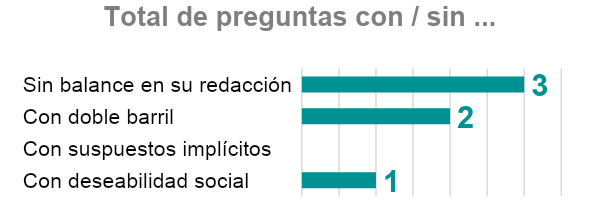
\includegraphics[width=12cm]{figures/61uGdr.png}
\end{center}

\begin{center}
    \begin{mybox}[colback=white, width = 7cm]{equation*}
      \text{Número total de preguntas: }
    \end{mybox}
\end{center}

\begin{center}
  \begin{mybox}[colback=white, width = 7cm]{equation*}
    Observaciones generales sobre las preguntas \\
    \\
  \end{mybox}
\end{center}

\newpage

\subsection{Anáisis general de opciones de respuesta}

\begin{center}
    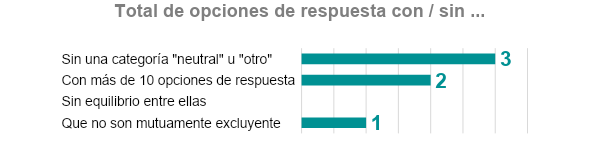
\includegraphics[width=13cm]{figures/Caftsq.png} 
    \begin{mybox}[colback=white, width = 7cm]{equation*}
    Observaciones generales sobre las respuestas \\
    \\
    \end{mybox}
\end{center}

\section{Análisis por bloque}

\begin{center}
    \begin{tabular}{ c  c }
      \begin{mybox}[colback=white, width = 7cm]{equation*}
      Nombre del bloque: 
      \end{mybox}
      & 
      \begin{mybox}[colback=white, width = 7cm]{equation*}
      Número total de preguntas: 
      \end{mybox}
    \end{tabular}
\end{center}

\medskip

\begin{center}
  \begin{tabularx}{\textwidth}[t]{XXX}
    \arrayrulecolor{black}\hline
      \textbf{\textcolor{amarillom}{Anáisis de preguntas.}} & \\ \hline
        & Número & Observación \\ \hline
      \begin{minipage}[t]{\linewidth}%
        \begin{itemize}
          \item Número de preguntas con deseabilidad social \\
        \end{itemize} 
      \end{minipage} & & \\ \hline
      \begin{minipage}[t]{\linewidth}%
        \begin{itemize}
          \item Número de preguntas con supuestos implícitos \\
        \end{itemize} 
      \end{minipage} & & \\ \hline
      \begin{minipage}[t]{\linewidth}%
        \begin{itemize}
          \item Número de preguntas con doble barril \\
        \end{itemize} 
      \end{minipage} & & \\ \hline
      \begin{minipage}[t]{\linewidth}%
        \begin{itemize}
          \item Número de preguntas sin balance en su redacción \\
        \end{itemize} 
      \end{minipage} & & \\ \hline
  \arrayrulecolor{black}\hline
  \end{tabularx}
\end{center}

\begin{center}
    \begin{tabularx}{\textwidth}[t]{XXX}
      \arrayrulecolor{black}\hline
      \textbf{\textcolor{amarillom}{Anáisis de opciones de respuesta.}} & \\ \hline
        & Número & Observación \\ \hline
      \begin{minipage}[t]{\linewidth}%
        \begin{itemize}
          \item Número de preguntas con opciones de respuesta que no son mutuamente excluyentes\\
        \end{itemize} 
      \end{minipage} & & \\ \hline
      \begin{minipage}[t]{\linewidth}%
        \begin{itemize}
          \item Número de preguntas con opciones de respuesta sin equilibrio entre ellas\\
        \end{itemize} 
      \end{minipage} & & \\ \hline
      \begin{minipage}[t]{\linewidth}%
        \begin{itemize}
          \item Número de preguntas que tienen más de 10 opciones de respuesta\\
        \end{itemize} 
      \end{minipage} & & \\ \hline
      \begin{minipage}[t]{\linewidth}%
        \begin{itemize}
          \item Número de preguntas que necesitan una categoría de respuesta “neutral” o la opción de “otro” y no cuentan con ella \\
      \end{itemize} 
    \end{minipage} & & \\ \hline
    \arrayrulecolor{black}\hline
\end{tabularx}
\end{center}
\newpage

\section{Análisis de formularios}

\begin{figure}[!htb]
  \begin{minipage}{0.3\textwidth}
    \centering

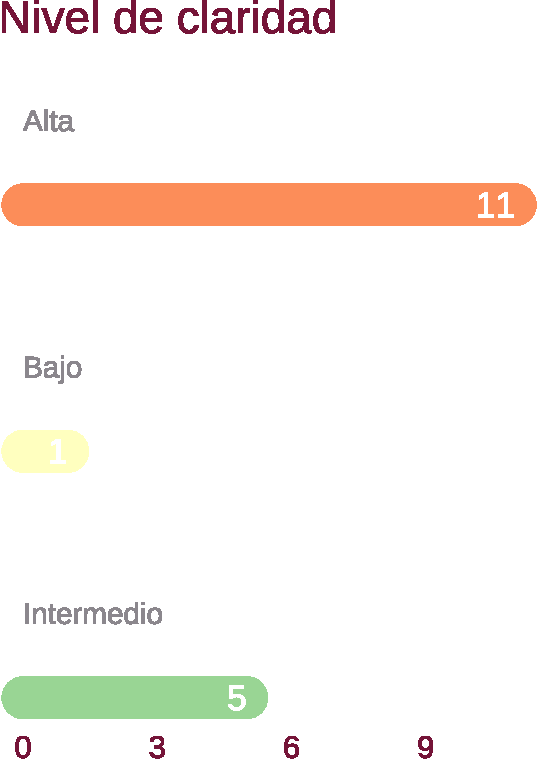
\includegraphics[width=\textwidth]{ReportEncuestaElectoral_files/figure-latex/unnamed-chunk-1-1} 
  \end{minipage}\hfill
  \begin{minipage}{0.3\textwidth}
    \centering

\includegraphics[width=\textwidth]{ReportEncuestaElectoral_files/figure-latex/unnamed-chunk-2-1} 
  \end{minipage}
    \begin{minipage}{0.3\textwidth}
    \centering

\includegraphics[width=\textwidth]{ReportEncuestaElectoral_files/figure-latex/unnamed-chunk-3-1} 
  \end{minipage}
\end{figure}

\begin{figure}[!htb]
  \begin{minipage}{0.3\textwidth}
    \centering

\includegraphics[width=\textwidth]{ReportEncuestaElectoral_files/figure-latex/unnamed-chunk-4-1} 
  \end{minipage}\hfill
  \begin{minipage}{0.3\textwidth}
    \centering

\includegraphics[width=\textwidth]{ReportEncuestaElectoral_files/figure-latex/unnamed-chunk-5-1} 
  \end{minipage}
  \\
  \centering
  \begin{minipage}{0.3\textwidth}
    \centering

\includegraphics[width=\textwidth]{ReportEncuestaElectoral_files/figure-latex/unnamed-chunk-6-1} 
  \end{minipage}
\end{figure}

\newpage

\section{Análisis de diseño muestral}

\begin{figure}[!htb]
    \begin{minipage}{0.5\textwidth}
      \centering

\includegraphics[width=\textwidth]{ReportEncuestaElectoral_files/figure-latex/unnamed-chunk-7-1} 
    \end{minipage}\hfill
    \begin{minipage}{0.5\textwidth}
      \centering

\includegraphics[width=\textwidth]{ReportEncuestaElectoral_files/figure-latex/unnamed-chunk-8-1} 
    \end{minipage}
\end{figure}

\begin{figure}[!htb]
  \begin{minipage}{0.3\textwidth}
    \centering

\includegraphics[width=\textwidth]{ReportEncuestaElectoral_files/figure-latex/unnamed-chunk-9-1} 
    \end{minipage}\hfill
  \begin{minipage}{0.3\textwidth}
    \centering

\includegraphics[width=\textwidth]{ReportEncuestaElectoral_files/figure-latex/unnamed-chunk-10-1} 
  \end{minipage}
\end{figure}

\begin{figure}[!htb]
  \begin{minipage}{0.3\textwidth}
    \centering

\includegraphics[width=\textwidth]{ReportEncuestaElectoral_files/figure-latex/unnamed-chunk-11-1} 
  \end{minipage}\hfill
  \begin{minipage}{0.3\textwidth}
    \centering

\includegraphics[width=\textwidth]{ReportEncuestaElectoral_files/figure-latex/unnamed-chunk-12-1} 
  \end{minipage}
    \begin{minipage}{0.3\textwidth}
    \centering

\includegraphics[width=\textwidth]{ReportEncuestaElectoral_files/figure-latex/unnamed-chunk-13-1} 
  \end{minipage}
\end{figure}

\newpage

\begin{figure}[!htb]
\centering
  \begin{minipage}{0.3\textwidth}
    \centering

\includegraphics[width=\textwidth]{ReportEncuestaElectoral_files/figure-latex/unnamed-chunk-14-1} 
  \end{minipage}\hfill
\end{figure}

\begin{figure}[!htb]
  \begin{minipage}{0.3\textwidth}
  \centering

\includegraphics[width=\textwidth]{ReportEncuestaElectoral_files/figure-latex/unnamed-chunk-15-1} 

  \end{minipage}\hfill
  \begin{minipage}{0.3\textwidth}
    \centering

\includegraphics[width=\textwidth]{ReportEncuestaElectoral_files/figure-latex/unnamed-chunk-16-1} 
  \end{minipage}
  \\
  \centering
  \begin{minipage}{0.3\textwidth}
    \centering

\includegraphics[width=\textwidth]{ReportEncuestaElectoral_files/figure-latex/unnamed-chunk-17-1} 
\end{minipage}
\end{figure}

\newpage

\section{Analysis Report}

\subsection{Subtitle}

Lorem ipsum dolor sit amet, consectetur adipiscing elit. Donec nec
fermentum augue. Integer id neque sit amet augue lacinia fringilla.
Donec leo ipsum, dapibus vel orci et, viverra viverra sem. Morbi maximus
neque ipsum, in vulputate libero porta a. Interdum et malesuada fames ac
ante ipsum primis in faucibus. Nulla at libero arcu.

\begin{figure}[htb]
  \centering
  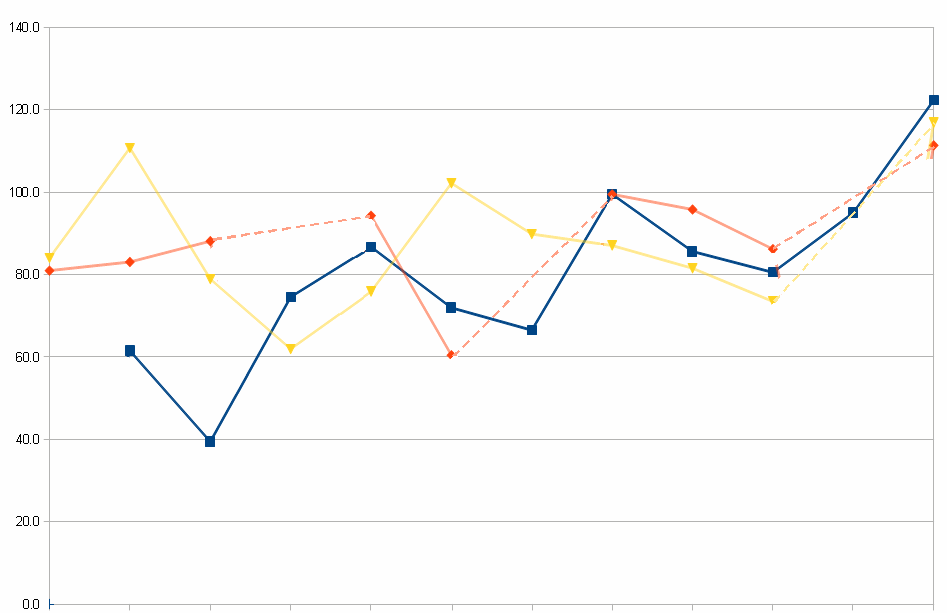
\includegraphics[width=1\textwidth]{figures/figure1.png}
  \centering
\end{figure}

\subsubsection{Subsection}

In pretium enim dui, quis ornare odio varius et. Nulla facilisi. Nunc
tristique tortor at urna vehicula, elementum bibendum tortor hendrerit.
Ut eu risus nisi. Vestibulum nunc lorem, tristique sed ultrices nec,
porta et ligula. Nam facilisis felis a congue auctor. Fusce id odio in
libero blandit cursus nec nec arcu. Nulla eu ultricies massa, id dapibus
nisi. Donec tellus urna, maximus nec semper id, consectetur eu mi.
Vestibulum elit eros, porta ac eros a, mattis pulvinar magna. Nulla
pellentesque dapibus leo molestie varius. Duis ut rutrum urna, at
condimentum dui. Sed orci magna, faucibus nec quam et, malesuada
ultrices velit. Nam a lorem a massa facilisis rutrum eget id nunc. Morbi
aliquet felis et tincidunt scelerisque.


\end{document}
